
\begin{figure}
    \centering
    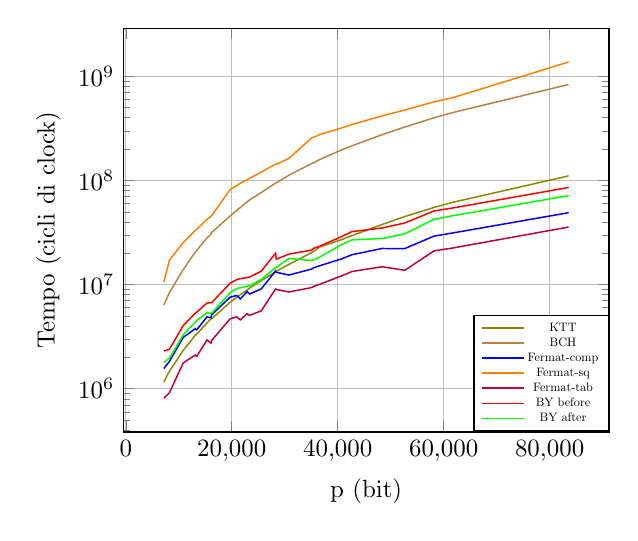
\begin{tikzpicture}[scale=0.9]
        \pgfplotsset{every axis/.append style={semithick}, legend style={nodes={scale=0.7, transform shape}, at={(1,0)},anchor=south east}}

	\begin{semilogyaxis}[
		xlabel=p (bit),ylabel=Tempo (cicli di clock), grid=major, xticklabel style={
            /pgf/number format/fixed,
            /pgf/number format/precision=5
            }, scaled x ticks=false ]

    \addplot[no marks, color=olive] coordinates{
        (7187, 1159197.4)
        (8237, 1469920.2)
        (10853, 2336473.4)
        (13109, 3246316.8)
        (13397, 3347390.0)
        (15331, 4277250.6)
        (16067, 4695806.2)
        (16229, 4694091.6)
        (19709, 6764716.4)
        (20981, 7556269.0)
        (21611, 8000344.2)
        (22901, 8858165.2)
        (23371, 9267820.8)
        (25579, 10906522.6)
        (28277, 13221080.6)
        (28411, 13423327.6)
        (30803, 15622464.4)
        (35117, 20323059.0)
        (35507, 20936273.0)
        (36629, 22957209.2)
        (40787, 27063629.4)
        (42677, 29510000.0)
        (48371, 37725077.4)
        (52667, 45033239.4)
        (58171, 54986958.0)
        (61717, 61625946.6)
        (83579, 110553683.6)
    };
    \addlegendentry{KTT}

    \addplot[no marks, color=brown] coordinates{
        (7187, 6368874.4)
        (8237, 8364095.6)
        (10853, 13922595.2)
        (13109, 20491931.0)
        (13397, 21293264.8)
        (15331, 28056795.4)
        (16067, 30382587.2)
        (16229, 31722889.2)
        (19709, 45575386.6)
        (20981, 51657051.6)
        (21611, 54956980.4)
        (22901, 62186967.6)
        (23371, 64996685.6)
        (25579, 76589311.4)
        (28277, 94263290.2)
        (28411, 94610992.2)
        (30803, 112420385.4)
        (35117, 145454923.6)
        (35507, 148202625.6)
        (36629, 158941209.0)
        (40787, 196929065.2)
        (42677, 214790361.0)
        (48371, 274893671.4)
        (52667, 325854983.0)
        (58171, 399131155.0)
        (61717, 448249901.0)
        (83579, 834007747.8)
    };
    \addlegendentry{BCH}

    \addplot[no marks, color=blue] coordinates {
        (7187, 1561699.8)
        (8237, 1827586.0)
        (10853, 3110983.6)
        (13109, 3770875.2)
        (13397, 3678711.8)
        (15331, 4900348.2)
        (16067, 4806660.2)
        (16229, 5133151.8)
        (19709, 7576635.0)
        (20981, 7857809.2)
        (21611, 7268007.2)
        (22901, 8562007.6)
        (23371, 8120296.6)
        (25579, 9097204.4)
        (28277, 13504138.2)
        (28411, 13120726.4)
        (30803, 12347247.6)
        (35117, 14105630.4)
        (35507, 14518979.4)
        (36629, 15177688.2)
        (40787, 17682828.6)
        (42677, 19342802.0)
        (48371, 22206770.4)
        (52667, 22177420.0)
        (58171, 29189824.2)
        (61717, 31306422.6)
        (83579, 48987526.4)
    };
    \addlegendentry{Fermat-comp}

    \addplot[no marks, color=orange] coordinates{
        (7187, 10597590.4)
        (8237, 17184007.0)
        (10853, 25297424.2)
        (13109, 33119433.8)
        (13397, 34034539.2)
        (15331, 42226171.0)
        (16067, 45221734.2)
        (16229, 46011999.6)
        (19709, 81895383.8)
        (20981, 89587471.2)
        (21611, 94080496.0)
        (22901, 101717262.2)
        (23371, 105224090.2)
        (25579, 119787535.4)
        (28277, 143408586.6)
        (28411, 142583988.2)
        (30803, 163023836.2)
        (35117, 256737134.2)
        (35507, 261421235.4)
        (36629, 274770918.6)
        (40787, 320387425.4)
        (42677, 343968765.2)
        (48371, 417034409.0)
        (52667, 474298878.0)
        (58171, 568372615.0)
        (61717, 623609013.0)
        (83579, 1370972271.0)        
    };
    \addlegendentry{Fermat-sq}
    
    \addplot[no marks, color=purple] coordinates {
        (7187, 809715.8)
        (8237, 915526.2)
        (10853, 1771415.4)
        (13109, 2103486.2)
        (13397, 2047749.8)
        (15331, 2939877.8)
        (16067, 2740291.6)
        (16229, 2917695.0)
        (19709, 4695404.2)
        (20981, 4895648.2)
        (21611, 4576126.0)
        (22901, 5257624.8)
        (23371, 5057833.2)
        (25579, 5597524.4)
        (28277, 9083607.2)
        (28411, 8978193.0)
        (30803, 8485064.2)
        (35117, 9378049.2)
        (35507, 9621184.2)
        (36629, 10076641.2)
        (40787, 12150942.0)
        (42677, 13344390.2)
        (48371, 14827613.0)
        (52667, 13711557.0)
        (58171, 21056187.8)
        (61717, 22448997.0)
        (83579, 35664757.6)        
    };
    \addlegendentry{Fermat-tab}

    \addplot[no marks, color=red] coordinates {
		(7187, 2301133.4)
        (8237, 2390625.0)
        (10853, 4044599.2)
        (13109, 5300937.4)
        (13397, 5446870.6)
        (15331, 6648405.6)
        (16067, 6702943.8)
        (16229, 6724461.8)
        (19709, 10310837.6)
        (20981, 11196952.2)
        (21611, 11407319.0)
        (22901, 11667615.0)
        (23371, 11805428.0)
        (25579, 13449986.4)
        (28277, 20024899.6)
        (28411, 17511886.6)
        (30803, 19631753.0)
        (35117, 21432919.4)
        (35507, 22369455.6)
        (36629, 23348801.4)
        (40787, 28987888.4)
        (42677, 32262773.2)
        (48371, 34922057.2)
        (52667, 39038512.2)
        (58171, 50907356.2)
        (61717, 54401236.2)
        (83579, 85570203.0)
    };
    \addlegendentry{BY before}

    \addplot[no marks, color=green] coordinates {
        (7187, 1782584.6)
        (8237, 1962955.5)
        (10853, 3299358.6)
        (13109, 4362019.9)
        (13397, 4522305.42)
        (15331, 5368479.5)
        (16067, 5286806.16)
        (16229, 5325745.7)
        (19709, 8352941.2)
        (20981, 9162305.2)
        (21611, 9307480.6)
        (22901, 9655103.68)
        (23371, 9723034.62)
        (25579, 11202767.42)
        (28277, 14555232.2)
        (28411, 14622453.44)
        (30803, 17820851.56)
        (35117, 17008580.68)
        (35507, 17287261.4)
        (36629, 18419434.4)
        (40787, 24264261.8)
        (42677, 26849432.52)
        (48371, 27695913.8)
        (52667, 30734590.3)
        (58171, 42328589.2)
        (61717, 45814829.52)
        (83579, 71488995.4)        
    };
    \addlegendentry{BY after}

    \end{semilogyaxis}%
\end{tikzpicture}%
\caption{Tempi di esecuzione}
\end{figure}